\documentclass{jsarticle} %図が見づらかったのでjsarticleにしました

\usepackage{graphicx}
\usepackage{url}
\usepackage{listings,jlisting}
\usepackage{ascmac}
\usepackage{amsmath,amssymb}

%ここからソースコードの表示に関する設定
\lstset{
  basicstyle={\ttfamily},
  identifierstyle={\small},
  commentstyle={\smallitshape},
  keywordstyle={\small\bfseries},
  ndkeywordstyle={\small},
  stringstyle={\small\ttfamily},
  frame={tb},
  breaklines=true,
  columns=[l]{fullflexible},
  numbers=left,
  xrightmargin=0zw,
  xleftmargin=3zw,
  numberstyle={\scriptsize},
  stepnumber=1,
  numbersep=1zw,
  lineskip=-0.5ex
}
%ここまでソースコードの表示に関する設定

\title{知能プログラミング演習II 課題4}
\author{グループ7\\
  29114048 北原 太一\\
%  {\small (グループレポートの場合は、グループ名および全員の学生番号と氏名が必要)}
}
\date{2019年11月18日}

\begin{document}
\maketitle

\subparagraph{提出物} rep4
\subparagraph{グループ} グループ7
\subparagraph{メンバー}
\begin{tabular}{|c|c|c|}
  \hline
  学生番号&氏名&貢献度比率\\
  \hline\hline
  29114007&池口弘尚&100\\
  \hline
  29114031&大原拓人&100\\
  \hline
  29114048&北原太一&100\\
  \hline
  29114086&飛世裕貴&100\\
  \hline
  29114095&野竹浩二朗&100\\
  \hline
\end{tabular}

\section{課題の説明}
\begin{description}
\item[課題4-1] まず,教科書3.2.1の「前向き推論」のプログラムと教科書3.2.2の「後向き推論」のプログラムとの動作確認をし,前向き推論と後ろ向き推論の違いを説明せよ.
  また,実行例を示してルールが選択される過程を説明せよ.
  説明の際には,LibreOfficeのDrawなどのドロー系ツールを使ってp.106図3.11やp.118図3.12のような図として示すことが望ましい.
\item[課題4-2] CarShop.data , AnimalWorld.data等のデータファイルを実際的な応用事例に書き換えて,前向き推論,および後ろ向き推論に基づく質問応答システムを作成せよ.
  なお,ユーザの質問は英語や日本語のような自然言語が望ましいが,難しければ変数を含むパターン等でも可とする.
\item[課題4-3] 上記4-2で実装した質問応答システムのGUIを作成せよ.
  質問に答える際の推論過程を可視化できることが望ましい.
\item[課題4-4] 上記4-3で実装したGUIを発展させ,質問応答だけでなく,ルールの編集などについてもGUIで行えるようにせよ.
\end{description}


\section{課題4-1}
\begin{screen}
 まず,教科書3.2.1の「前向き推論」のプログラムと教科書3.2.2の「後向き推論」のプログラムとの動作確認をし,前向き推論と後ろ向き推論の違いを説明せよ.
  また,実行例を示してルールが選択される過程を説明せよ.
  説明の際には,LibreOfficeのDrawなどのドロー系ツールを使ってp.106図3.11やp.118図3.12のような図として示すことが望ましい.
\end{screen}

\subsection{前向き推論}

まず、デフォルトのまま前向き推論のRuleBaseSystem.javaを実行した時における推論過程を図\ref{fig:FCCS}に示す。なお、一番上の点線で囲まれたアサーションは元々ワーキングメモリ上にあることを表す。

 \begin{figure}[htbp]
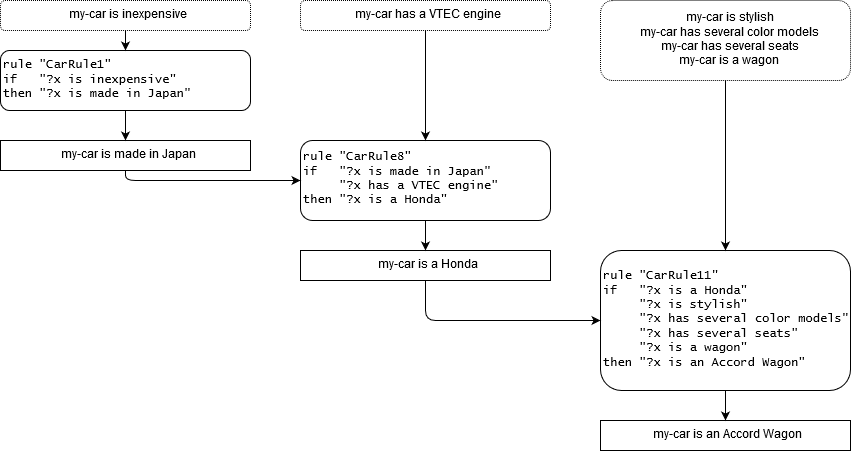
\includegraphics[bb=0 0 401 532,width=0.48\linewidth]{Forward1.png}
\caption{前向き推論:CarShop.data}
\label{fig:FCCS}
\end{figure}

次に、AnimalWorld.dataを利用するためにRuleBaseSystem.javaのRuleBaseクラスのコンストラクタの一部をソースコード\ref{lst:FCAW}のように変えた。

  \begin{lstlisting}[caption=RuleBase2.java(一部抜粋),label=lst:FCAW]
fileName = "AnimalWorld.data";
wm = new WorkingMemory();
wm.addAssertion("my-friend has hair");
wm.addAssertion("my-friend eats meat");
wm.addAssertion("my-friend has tawny color");
wm.addAssertion("my-friend has black");
  \end{lstlisting}
  
このプログラムを実行した時における推論過程を図\ref{fig:FCAW}に示す。
 
\begin{figure}[htbp]
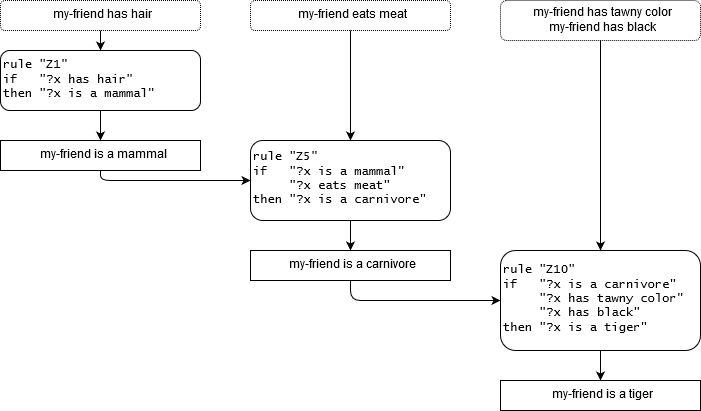
\includegraphics[bb=0 0 401 532,width=0.57\linewidth]{Forward2.png}
\caption{前向き推論:AnimalWorld.data}
\label{fig:FCAW}
\end{figure}

\pagebreak
\subsection{後向き推論}

まず、デフォルトのまま後向き推論のRuleBaseSystem.javaをソースコード\ref{lst:BCCS}に示すコマンドで実行した。

\begin{lstlisting}[caption=後ろ向き推論1,label=lst:BCCS]
>java RuleBaseSystem "?x is an Accord Wagon"
\end{lstlisting}

この実行における推論過程を図\ref{fig:BCCS}に示す。なお、矢印の隣の括弧つき数字はルールの適用順を、(WM)はワーキングメモリ上のアサーションを、矢印上の×印はワーキングメモリ上のアサーションと一致しなかったことを表す。

\begin{figure}[htbp]
%jarticleでこの通りにすると小さすぎて読めません
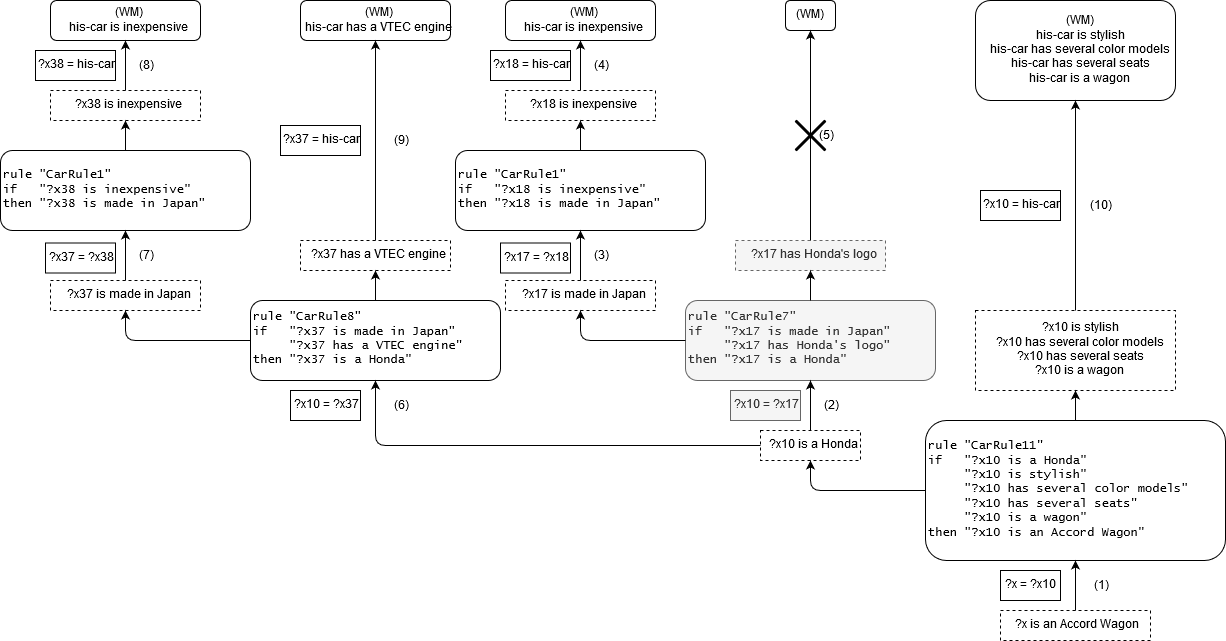
\includegraphics[bb=0 0 401 532,width=0.34\linewidth]{Backward1.png}
\caption{後向き推論:CarShop}
\label{fig:BCCS}
\end{figure}

\pagebreak
次に、デフォルトのRuleBaseSystem.javaのコメントアウトを付け替え、CarShop.data, CarShopWm.dataの代わりにAnimalWorld.data, AnimalWorldWm.dataを使用するようにしたうえでソースコード\ref{lst:BCAW}に示すコマンドを実行した。

\begin{lstlisting}[caption=後向き推論2,label=lst:BCAW]
>java RuleBaseSystem "?x is giraffe"
\end{lstlisting}

この実行における推論過程をCarShopの場合と同じように図\ref{fig:BCAW}に示す。

\begin{figure}[htbp]
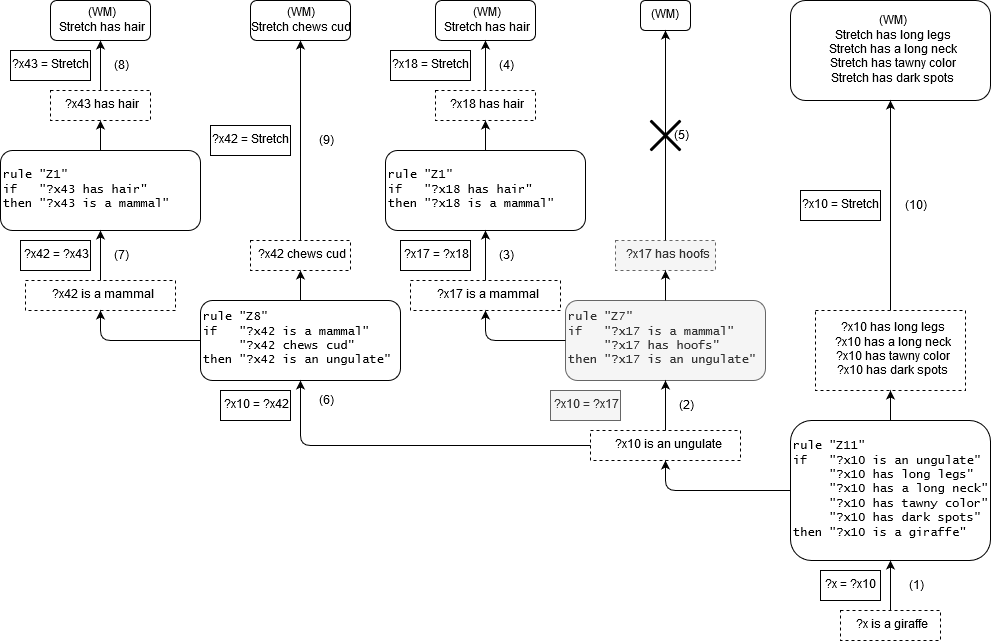
\includegraphics[bb=0 0 401 532,width=0.41\linewidth]{Backward2.png}
\caption{後向き推論:AnimalWorld}
\label{fig:BCAW}
\end{figure}

\pagebreak
\subsection{考察}

前向き推論では、すでにワーキングメモリ上にあるアサーションからルールを適用して新しいアサーションを導く。すなわち、すでにある知識から新しい知識を導く手法といえる。また、後向き推論では、与えられたパターンにルールを適用し、新しいパターンを作り、最後にワーキングメモリ上のパターンとマッチングさせる。すなわち、仮定にどの知識が合致する、あるいは当てはまるかを導く手法といえる。\\
 この両者の大きな違いとして、ワーキングメモリの使い方を挙げることができる。すなわち、前向き推論においてはワーキングメモリが推論のスタート地点であり、後向き推論においてはワーキングメモリが推論のゴール地点である。

\section{参考文献}

新谷虎松,講義「知識システム」スライド

\end{document}
